%% $Id$

\documentclass[a4paper,10pt,bibtotoc]{scrartcl}
\usepackage{a4wide,usg,supertabular}
\usepackage[today,nofancy]{svninfo}
%\usepackage[colorlinks=true,urlcolor=cyan]{hyperref}

\svnInfo $Id$

\begin{document}

%%_______________________________________________________________________________
%%                                                                      Titlepage

\title{LOFAR User Guide: \\ The Framework Pulsar Pipeline\\
{\large Pulp, Version 1.0} \\ 
{\normalsize Document version 1.0} \\
{\normalsize SVN Repository Revision: \svnInfoRevision}}
\author{K. R. Anderson}
\date{\small{SVN Date: \svnInfoDate}}
\maketitle

\tableofcontents

\clearpage

%%_______________________________________________________________________________
%%                                                                  Change record

\section*{Change record}
\addcontentsline{toc}{section}{Change record}

\begin{center}
  %% Table head
  \tablefirsthead{
    \hline
    \sc Issue & \sc Date & \sc Sections & \sc Description of changes \\
    \hline
  }
  \tablehead{
    \multicolumn{4}{r}{\small\sl continued from previous page} \\
    \hline
    \sc Issue & \sc Date & \sc Sections & \sc Description of changes \\
    \hline
  }
  %% Table tail
  \tabletail{
    \hline
    \multicolumn{4}{r}{\small\sl continued on next page} \\
  }
  \tablelasttail{\hline}
  %% Table contents
  \begin{supertabular}{lllp{10cm}}
    1.0 & 2011-01-31 & all & Initial release \\
  \end{supertabular}
\end{center}
\clearpage

%%_______________________________________________________________________________
%%                                                                   Introduction

\section{Introduction}
\label{sec:introduction}
\verb|>>> import| This document is version 1.0 of the LOFAR User Guide for the LOFAR
framework pulsar pipeline, known colloquially as `pulp'.  This User
Guide provides general instruction to help users establish a viable user environment
as required by the LOFAR pipeline framework in order to run
the framework pulsar pipeline in the LOFAR cluster compute environment.

This document will also present details on running the
framework pulsar pipeline, known as Pulp (executable: \verb|pulp.py|).
Users are encouraged to seek detailed information about the
actual processing engaged by the ``known pulsar pipeline'' from the
LOFAR Transient Key Project (TKP) science team. Details
regarding LOFAR beam-formed data processing actual are beyond the scope of this
document.\footnote{Readers of this
  document who find themselves unfamiliar with the terms, `known pulsar
  pipeline,'  or `Jason Hessels', should probably be reading something else.}

This document assumes some familiarity with terms surrounding the pipeline
framework, such as ``recipe'',  and ``head node'', as well as terms
associated with ``known pulsar pipeline'' processing. Such terms will
be used throughout this document.

\subsection{Applicable Documents}
Documentation on the Pulp package is provided with the Pulp
distribution, and is available with the Pulp package download in
\verb|${LOFARSOFT}/src/Pulsar/pipeline/documentation|\footnote{This
  document can be found op ``UserGuide/UserGuide.pdf','' under
  ``documentation/''}. Further documentation on the LOFAR pipeline
framework, development under the LOFAR pipeline framework,  as well as schematic
documentation on the Pulp API, are available within the repository
itself. Pulp API documents are delivered with the Pulp package as
part of any download of the \verb|$LOFARSOFT| repository.

The Pulp current release under the LOFAR USG repository is located in \\
\noindent \verb|$LOFARSOFT/src/Pulsar/pipeline:|
\begin{verbatim}
drwxr-xr-x   9 <user>    staff     306 Feb  2 18:07 .svn 
-rw-r--r--@  1 <user>    staff      67 Jan 31 01:29 __init__.py
drwxr-xr-x   8 <user>    staff     272 Feb  2 18:05 documentation/
-rw-r--r--   1 <user>    staff    3614 Jan 28 20:33 dynspec.py
-rw-r--r--   1 <user>    staff    1708 Jan 21 17:16 pipeline.cfg
-rwxr-xr-x   1 <user>    staff    4545 Jan 31 01:48 pulp.py
rw-r--r--    1 <user>    staff      40 Jan 28 17:28 pulpVersion.py
drwxr-xr-x   6 <user>    staff     204 Jan 31 01:21 recipes/
drwxr-xr-x  18 <user>    staff     612 Feb  1 16:16 support/
-rw-r--r--   1 <user>    staff     789 Jan 28 22:07 tasks.cfg
\end{verbatim}
In \verb|documentation/|, users will  find a directory structure that
somewhat mimics the pipeline's recipe-support directory structure, with
recipe API documents found under
\verb|./pipeline/documentation/PulpAPI/| in
`master',`nodes', and `support', which contain, respectively, head
node recipes, compute node recipes, and support modules providing adminstrative and
executive function.
\begin{verbatim}
$LOFARSOFT src/Pulsar/pipeline/documentation:

  drwxr-xr-x   9 <user>     staff  306 Jan 30 08:08 .svn
  drwxr-xr-x   6 <user>     staff  204 Feb  3 15:09 PulpAPI
  drwxr-xr-x  27 <user>     staff  918 Feb  3 00:00 UserGuide
\end{verbatim}
where a user will find API documents for the pipeline recipes, and all support
modules.\\
\begin{verbatim}
./PulpAPI/master:
-------
-rw-r--r--@   0  __init__.py
 rw-r--r--  ...  bf2presto.html
-rw-r--r--  ...  buildPulsArch.html
-rw-r--r--  ...  buildRSPAll.html
-rw-r--r--  ...  bundleFiles.html
-rw-r--r--  ...  prepareInf.html
-rw-r--r--  ...  prepfold.html
-rw-r--r--  ...  rfiplot.html

./PulpAPI/nodes:
------
-rw-r--r--@   0 __init__.py
-rw-r--r--  ...  bf2presto.html
-rw-r--r--  ...  prepfold.html
-rw-r--r--  ...  rfiplot.html

./PulpAPI/support:
--------
-rw-r--r--@   0  __init__.py
 rw-r--r--  ...  RSPlist.html
-rw-r--r--  ...  bf2Pars.html
-rw-r--r--  ...  buildRSPS.html
-rw-r--r--  ...  bundlePlots.html
-rw-r--r--  ...  foldingData.html
-rw-r--r--  ...  fullRSP.html
-rw-r--r--  ...  pardata.html
-rw-r--r--  ...  prepInfFiles.html
-rw-r--r--  ...  pulpEnv.html
-rw-r--r--  ...  rfiDirectories.html
\end{verbatim}
These are accessible and viewable through any browser.

\subsection{Reference Documents}
For documentation on the framework itself, as well as guidance on recipe writing,
the user is invited to examine the framework documenation available in the 
repository under
\begin{verbatim}
${LOFARSOFT}/src/pipeline/docs .
\end{verbatim}
A subset of the framework's API is documented in the Pulp  API
documentation described above.

\subsection{Package Overview}
\label{sec:package}
The Pulp package is based upon the the LOFAR TKP Pulsar Group's pipelining shell 
script\footnote{ \texttt{make\_subs\_SAS\_Ncore\_Mmodes.sh} in
\texttt{ \$\{LOFARSOFT\}/lofarsoft/src/Pulsar/scripts}}.  Pulp is 
built on the LOFAR pipeline framework and, as with all such pipelines, 
comprises a set of `recipes' that are executed in successive order.  
In a cluster compute environment, these recipes can be paired in order 
to facilitate parallel processing on a cluster and/or subsections of a 
cluster. Depending upon the required action, recipes may or may not be 
paired across head node/compute node connections.\footnote{This is
  explicitly true for the Pulp package, as it employs the framework's IPython
  facility.  This statement is likely not correct for the ``new
  style'' imaging pipeline, which employs an ssh protocol.}  When a ``head node'' 
recipe is not paired with a matching ``compute node'' recipe (name
matching of head/compute node recipes is required by the framework),
this necessarily implies that a single process will be activited on a
compute node in order to perform a task that does not require
parallelization. For example, building the storage node directory
structure for an observation.

In order to illustrate this meaning, Table \ref{tab:recipeTable} presents 
the overall organisation of the Pulp pulsar pipeline package.  The table 
demonstrates those recipes that will perform the tasks requiring multiple 
parallel jobs.  Those recipes (bolded) show matching named ``node recipe'' 
modules in the package.  It is these head node/compute node recipe pairs that 
multiply execute all requested processing jobs.  Those jobs, and the resulting 
job queues, are arranged and built by the respective head node recipe, and 
then farmed to the cluster based upon a user's ``clusterdesc'' 
file (see \S \ref{sec:environment}).

\begin{table}[ht]
\centering
\begin{tabular}{|r|c|l|}
\hline
\textsc{Master Recipe} &\textsc{Node Recipe}&\textsc{Support Modules}\\
\hline \hline
buildPulsArch & --- & buildRSPS,RSPlist\\
\hline
    \textbf{bf2presto} & \textbf{bf2presto} & bf2Pars, pulpEnv\\
\hline
  buildRSPALL &    ---    & fullRSP, pulpEnv\\
\cline{1-2}
   prepareInf &    ---    & prepareInfFiles, pulpEnv\\
\hline
    \textbf{prepfold} & \textbf{prepfold}  & pulpEnv\\
\hline
      \textbf{rfiplot} &\textbf{rfiplot}   & rfiDirectories, pulpEnv\\
\hline
bundleFiles &    ---    & bundlePlots, pulpEnv\\
\hline
\end{tabular}
  \caption{Pulp distribution and recipe relations}
  \label{tab:recipeTable}
\end{table}

\underline{Note}: \verb|support/| modules may support other \verb|support/| modules. Recipes do not support other recipes.
\newline
As indicated earlier (\S \ref{sec:introduction}), the described Pulp package is delivered 
via checkout of the LOFAR USG code repository.

\subsubsection{Nominal Pulp Processing}
The nominal processing performed by the Pulp package involves,
\begin{itemize}
\item The number of subbands in a observation is entirely selected by the observer,
however, nominally 248 subbands of `incoherent' beam-formed data are
usually delivered and processed.  Currently, Pulp can only process
so-called  `incoherentstokes' beam-formed data.\footnote{Development
  on `coherentstokes' data processing tabled until beam-formed data
  type is written in conformance with the \textsc{lofar-usg-icd-003} specification}\footnote{see LOFAR document, \textit{LOFAR-USG-ICD-003,
    Beam-formed Data}, Alexov et al, ASTRON, 2010.}  
\item The pipeline is capable of handling any user selected ``splitting'' factor, i.e. the 
`filefactor' parameter within Pulp.  This factor is known as ``ncores'' in the pulsar
shell script.  Pulp places no restriction on what `filefactor' can be, though nominal
processing will usually dictate the default \verb|filefactor = 8|.
Because of this, users are encouraged to use judgment in <filefactor>
specification, when the default is not desired.
\item In the special case that a user select \verb|filefactor == 1|,
  No ``all'' processing will be done.  That is, no
  \verb|RSPA| is made, and no \verb|RSPA| processing, \emph{per se},
  occurs.  Output will appear in the expected `\verb|RSP0| directory. \verb|RSP0| is equivalent to  \verb|RSPA|, when \verb|filefactor=1|.
\item The shell script ``-rfi'' swtich is not a switch with Pulp (it
  could be made that way).  Pulp executes the relevent steps
  automatically and the products, a dynamic spectrum of the data and a
  so-called  ``.rffireport'' file, are bundled as a standard pipeline data
  product. 
\end{itemize}

Details on the Pulp command line interface are provided in
\S\ref{sec:interfaces}, ``Interfaces''.
\subsection{Glossary}
\begin{itemize}
\item \textbf{API} -- Application programming interface (!Anton Pannekoek Instituut).
\item \textbf{Compute node} -- One of an assigned number of cluster nodes 
configured for computing.  For LOFAR, these compute nodes have NFS connections 
to selected storage nodes, which is where both input and output data will be 
read from  and written to.  Within the context of the LOFAR pipeline framework, compute nodes
are often referred to simply as ``nodes''.
\item \textbf{Cluster} -- A multi-node computing cluster.
\item \textbf{Head node} -- The head (controlling) node of a cluster environment. In the LOFAR 
computing environment, the head node is lfe001.  (rumours of a second
``head node'' on the LOFAR cluster, ``lfe002'', have been reported,
though remain confirmed by this user)
\item \textbf{Pulp} -- the ``known pulsar pipeline'' implemented under
  the LOFAR pipeline framework.
\item \textbf{TKP}-- The Transient Key Project (LOFAR).
\end{itemize}


\section{User Environment}
\label{sec:environment}
In computing environments, pipelines function as automated, simulated
users at the command line.  More aptly, a pipeline
functions as a proxy user, or user agent. Therefore, and in order
that the Pulp package execute properly, Pulp users will need to take a
number of steps in adjusting their compute environments. Framework
pipeline operations require that a number of locally defined
configuration files be accessible to the framework. These files are
(in no particular order):
\begin{enumerate}
\item pipeline.cfg            -- configuration for framework operations
\item tasks.cfg                -- define things to do
\item sub[n].clusterdesc -- define target compute nodes
\item task.furl                 -- job control
\item multiengine.furl     -- ip engine control
\end{enumerate}
The two configuration files, \verb|pipeline.cfg| and \verb|tasks.cfg|,
listed here are provided with the Pulp download.  Described below,
users will want to edit the pipeline configuration file to use their
own builds of the \verb|$LOFARSOFT| code repository.  Users may edit the
\verb|tasks.cfg| file, which is where a user may easily change default
arguments of any or all recipes.  In all likelihood, most users will
not want or need to do this. These configuration files, and others,
are discussed in detail in \S\ref{sec:cfgfiles}, ``Framework configuration files''.

\subsection{Configuration}
\label{sec:config}
\subsubsection{Environment variables, paths}

The following steps should be taken by users to establish the
environment  variables and directories required by the pipeline framework.
\begin{itemize}
\item[--] Define \verb|LOFARSOFT|, \verb|LOFARROOT (=/opt/LofIm/daily/lofar)|
\item [--]source \verb|${LOFARSOFT}/devel_common/scripts/init.sh|
\item [--]\verb|Use LofIm|
\item[--] Make a ``\verb|pipeline_runtime/|'' directory (arbitrary location)
\item[--] Edit user's \verb|pipeline.cfg| file to reflect this path
\item[--] Adjust \verb|$PYTHONPATH| to include framework python
  libraries.
\end{itemize}
Invocation of `\verb|Use LofIm|' will define the environment variables, \verb|$TEMPO|,
and \verb|$PRESTO|, needed for embedded
PRESTO\footnote{\texttt{http://www.cv.nrao.edu/-sransom/presto}} operations.

Users will need to make a directory the framework expects to use for
pipeline activities, such as writing various log files. Within the
above mentioned  configuration file, \verb|`pipeline.cfg'|, discussed in detail below,
users will define the configuration parameter, \verb|`runtime_directory'|.\\
i.e. 
\begin{verbatim}
runtime_directory = /path/to/your/runtime_directory
\end{verbatim}

As illustrated, this directory is arbitrary in both name and location,
though by convention, it is usually located under a user's home
directory.\footnote{Explicit paths must appear in this configuration file.}

Once these are defined (usually within a user's shell resource file),
a user's \verb|$PYTHONPATH| should further include the following paths
described below.  This should become obsolete in the near future
(v1.1), with refactoring to use package namespace explicivity, rather
than some still ``blind'' imports, usually on support modules).

\begin{verbatim}
PYTHONPATH=/opt/pipeline/dependencies/lib/python2.5/site-packages:\
/opt/pipeline/framework/lib/python2.5/site-packages:              \ 
/opt/LofIm/daily/pyrap/lib:                                       \
${LOFARROOT}/lib/python2.5/site-packages:                         \
/opt/pythonlibs/lib/python/site-packages:                         \
${LOFARSOFT}/src/Pulsar/pipeline/recipes/master:                  \
${LOFARSOFT}/src/Pulsar/pipeline/recipes/nodes:                   \
${LOFARSOFT}/src/Pulsar/pipeline/support 
\end{verbatim}

A user's \verb|$PATH| environment variable should be adjusted to include the following paths.

\verb|$PATH| include:
\begin{verbatim}
${LOFARSOFT}/release/bin:\ 
${LOFARSOFT}/release/share/pulsar/bin:\
${LOFARSOFT}/src/Pulsar/pipeline:\ 
/opt/LofIm/daily/casarest/bin:\ 
/opt/pipeline/dependencies/bin:\ 
/opt/LofIm/daily/askapsoft/bin:\ 
/opt/scripts:${PATH} 
\end{verbatim}
\underline{N.B.} These paths are subject to future alteration of the LOFAR system.

\subsubsection{Framework configuration files}
\label{sec:cfgfiles}
The pipeline framework functions through the use and availability of a limited set of configuration files, i.e., \verb|.cfg| files.  These configuration files are listed and briefly described.  For more information, see the documentation on the pipeline framework (Swinbank, 2011).\\
\begin{verbatim}
pipeline.cfg
tasks.cfg
\end{verbatim}
A user will notice that these two configuration files are delivered by
the svn repository.  These files are required by the framework.  They
are \emph{not} part of the Pulp package. Though they must be tailored by the
user to their particular environment and file system, the files are
provided by the repository as both convenience and necessity; the
\verb|pipeline.cfg| the convenience, the \verb|tasks.cfg| the necessity.

The \verb|pipeline.cfg| file is a ``pipeline generic'' configuration
file applicable to all framework pipelines.  The Pulp \verb|tasks.cfg|
file is not.  It is advised that this file not be altered without
perspicacious intent.

Here is the top level of a delivered \verb|$LOFARSOFT| Pulp directory:
\begin{verbatim}
[...]/lofarsoft/src/Pulsar/pipeline:
  drwxr-xr-x      .
  drwxr-xr-x      ..
  drwxr-xr-x      .svn
  -rw-r--r--@ ... __init__.py
  drwxr-xr-x  ... documentation/
  -rw-r--r--  ... dynspec.py
  -rw-r--r--  ... pipeline.cfg  ---> user paths and locations
  -rwxr-xr-x  ... pulp.py
  -rw-r--r--  ... pulpVersion.py
  drwxr-xr-x  ... recipes/
  drwxr-xr-x  ... support/
  -rw-r--r--  ... tasks.cfg     ---> task/recipe definitions
\end{verbatim}
The reasons these particular files are delivered as part of the Pulp
package are two fold: provide user's with a configuration basis, and
to specify Pulp functionality, delivered by the
\verb|tasks.cfg| file.  This confiuration file is critical to proper
pipeline operations and should not be altered by users unless done so
with understanding of pipeline operations.\\

Here is a quasi-generic pipeliine configuration file:
\begin{verbatim}
[DEFAULT]
runtime_directory  = /some/path/pipeline_runtime
recipe_directories = [<LOFARSOFTpath>/src/Pulsar/pipeline/recipes]
lofarroot          = /opt/LofIm/daily/lofar
default_working_directory = /data/scratch/<user>
task_files         = [<LOFARSOFTpath>/src/Pulsar/pipeline/tasks.cfg]


[layout]
job_directory     = %(runtime_directory)s/jobs/%(job_name)s
log_directory     = %(job_directory)s/logs/
vds_directory     = %(job_directory)s/vds
parset_directory  = %(job_directory)s/parsets
results_directory = %(job_directory)s/results/%(start_time)s


[cluster]
clustername      = pulsar
#clusterdesc     = %(runtime_directory)s/sub5.clusterdesc
clusterdesc      = %(runtime_directorypipe)s/line_runtime/sub6.clusterdesc
task_furl        = %(runtime_directory)s/task.furl
multiengine_furl = %(runtime_directory)s/multiengine.furl


[deploy]
script_path      = /opt/pipeline/framework/bin
controller_ppath = <LOFARSOFTpath>/src/Pulsar/pipeline/support:\
/opt/pipeline/dependencies/lib/python2.5/site-packages:\
/opt/pipeline/framework/lib/python2.5/site-packages

engine_ppath = <LOFARSOFTpath>/src/Pulsar/pipeline/recipes/master:\
<LOFARSOFTpath>//src/Pulsar/pipeline/recipes/node: \
<LOFARSOFTpath>/src/Pulsar/pipeline/support:
/opt/pipeline/dependencies/lib/python2.5/site-packages/:\
/opt/pipeline/framework/lib/python2.5/site-packages:\
/opt/LofIm/daily/pyrap/lib:\
/ot/LofIm/daily/lofar/lib/python2.5/site-packages:\
/opt/pythonlibs/lib/python/site-packages

engine_lpath = /opt/pipeline/dependencies/lib:\
/opt/LofIm/daily/pyrap/lib:\
/opt/LofIm/daily/casacore/lib:\
/opt/LofIm/daily/lofar/lib:\
/opt/wcslib/lib/:/opt/hdf5/lib

\end{verbatim}

The Pulp specific \verb|tasks.cfg| file is delivered with the Pulp
package. The set of  ``tasks'' are named within brackets, their names,
the names of available recipes.  The \verb|tasks.cfg| file is
specified in the \verb|pipeline.cfg| file.  Default recipe argument values
can be set in the \verb|tasks.cfg| file, as can be seen below.

\begin{verbatim}
[buildPulsArch]
recipe     = buildPulsArch
filefactor = 8

[bf2presto]
recipe     = bf2presto
executable = /home/kanderson/LOFAR/lofarsoft/release/share/pulsar/bin/bf2presto8
filefactor = 8
collapse   = False
nsigmas    = 7

[buildRSPAll]
recipe     = buildRSPAll
filefactor = 8

[prepareInf]
recipe     = prepareInf
filefactor = 8

[prepfold]
recipe     = prepfold
executable = /home/kanderson/LOFAR/lofarsoft/release/share/pulsar/bin/prepfold
filefactor = 8
nopdsearch = True
nperstokes = 256
noxwin     = True
fine       = True

[rfiplot]
recipe     = rfiplot
executable = /home/kanderson/LOFAR/lofarsoft/release/share/pulsar/bin/subdyn.py
filefactor = 8

[bundleFiles]
recipe     = bundleFilesj
filefactor = 8
\end{verbatim}
Users will note the explicit paths to \verb|$LOFARSOFT| executables.
This is because the configuration parser does not perform shell variable
interpolation\footnote{Rather disappointing}.  Upon Pulp download, users are encouraged to edit these explicit paths to use their own \verb|$LOFARSOFT| build.
\
\subsubsection{Cluster configuraton files}
Parallel processing as executed on the LOFAR offline cluster and through the pipeline framework will require three configuration files that define various parameters for job control on the LOFAR offline cluster.  None of these files are part of the Pulp distribution.  Users will have to locate templates of these files from the generalized pipeline framework location.  Once located, these files can be placed arbitrarily, with the arbitrary location specified in the above mentioned and critical \verb|pipeline.cfg| file.  Usually, these files are located in the user's specified ``runtime\_directory'', again defined in users' \verb|pipeline.cfg| files.
\begin{enumerate}
\item \verb|sub[n].clusterdesc| -- Cluster definition file.  Tells the framework how to use the cluster.
\item \verb|task.furl| -- furl file for tasks to be executed
\item \verb|multiengine furl| -- furl file for the multiengine client
\end{enumerate}
Of these files, the user will mostly likely edit the subcluster file, selecting compute node targets as needed.  An example of clusterdesc file content illustrates the configuration options.\\
\verb|sub5.clusterdesc|:
\begin{verbatim}
ClusterName = sub5 
# Storage nodes. 
Storage.Nodes         = [ lse013..15 ] 
Storage.LocalDisks    = [ /data1..4 ] 
# Compute nodes. 
Compute.Nodes         = [ lce037..45 ]         ==> selected compute nodes
Compute.RemoteDisks   = [ /net/sub1/lse013..15/data1..4 ] 
Compute.RemoteFileSys = [ /lse013..15:/data1..4 ] 
Compute.LocalDisks    = [ /data ] 
# Head nodes. 
Head.Nodes            = [ lfe001..2 ] 
Head.LocalDisks       = [ /data ]
\end{verbatim}
The most common adjustment user's might make here is altering the available ``Compute Nodes'' list, selecting or deslecting a subset of these ``sub5'' compute nodes.  As specified here, framework job control will (possibly) use all nodes on subnet five.


%%_______________________________________________________________________
%%                                                                                                           Interfaces

\section{Interfaces}
\label{sec:interfaces}
\subsection{Pulp command line interfaces}

\underline{(pulp.py, 1.0, delivered 31.01.2011)}

Once a user has established a viable environment for the framework pipeline, execution of Pulp should thence be straight forward.

The Pulp package provides two (2) pre-built command line interfaces
(``pre-built'' in the sense that users will certainly be writing their
own command line interfaces\footnote{Writing a
pipeline definition can be thought of as writing an interface to
control what processing the user wants done. Users should be
aware that, though the recipes are ``independent'', there is usually a
proxy dependence in that recipes may depend upon the
state of the data on disk as it may be provided by prior recipe calls}, that is,
their own pipeline definitions. The two defintions provided are
\begin{enumerate}
\item \verb|pulp.py|
\item \verb|dynspec.py|
\end{enumerate}

The pipeline definition \verb|pulp.py| runs the ``basic mode'' of the
``known pulsar pipeline.''\footnote{ \texttt{make\_subs\_SAS\_Ncore\_Mmodes.sh} in
\texttt{\$\{LOFARSOFT\}/lofarsoft/src/Pulsar/scripts}}. Users should
ensure \verb|PATH| access the this program. The ``cli'' to the
executable ``pulp.py'' module is invoked in the common pythonic idiom,\\

 i.e. \verb|$ python pulp.py -d --job-name ...|\\
\begin{verbatim}
 Current usage:

$ pulp.py --d --job-name=<job_name> --obsid=L<yyyy>_<nnnnn[...]>
--arch=<PULP_ARCHIVE> [--pulsar=<pulsar1[,pulsar2,pulsar3]>] [--filefactor=<m>]

where,

--d         = pipeline debug flag, full logging, use.
--obsid     = observation identifier          
--job-name  = arbitrary job name             
--arch      = selected PULSAR ARCHIVE.
--pulsar    = name of pulsar, or csv list of pulsar names.
              eg., --pulsar=B0919+06
                   --pulsar=B0919+06,B0834+06
filefactor  = subband splitting factor, <int>
              optional user specification (range, 1-248)
              default = 8
\end{verbatim}

The second interface provided is \verb|dynspec.py|, and was first
describe during the early November (2010) ``pulsar busy week''.  This
definition produces only the so-called ``rfi report'', and a `png'
image of the calculated dynamic spectrum, which is really
the product of the pulsar ``subdyn.py'' script\footnote{This python
  script can and should be refactored to be fully funtional on import.}.
The Pulp recipe stack is noticeably lighter sans prepfold.
\begin{verbatim}
Current usage:

$ dynspec.py --d --job-name=<job_name> --obsid=L<yyyy>_<nnnnn[...]>
--arch=<PULP_ARCHIVE> [--pulsar=<pulsar1[,pulsar2,pulsar3]>] [--filefactor=<m>]

where,

--d         = pipeline debug flag, full logging, use.
--obsid     = observation identifier          
--job-name  = arbitrary job name             
--arch      = selected PULSAR ARCHIVE.
--pulsar    = name of pulsar, or csv list of pulsar names.
              eg., --pulsar=B0919+06
                   --pulsar=B0919+06,B0834+06
filefactor  = subband splitting factor, <int>
              optional user specification (range, 1-248)
              default = 8
\end{verbatim}
\paragraph{The PULP\_ARCHIVE Device:}Users will find the data products of \verb|dynspec.py| located in the
various ``RSP[0-248]A'' directories\footnote{Though Pulp provides
  much more flexibilty in \textsc{rsp} splitting than the pulsar shell
  script, users are advised against using large numbers for
  filefactor, especially 248.  Mostly because, well, that just seems
  crazy.}, in the user selected Pulp archive (\verb|--arch=archnnn|) The user should be aware of the relationship between the defined subclusters of the offline LOFAR cluster, the electable storage nodes, and the location of the data.  For example, if a user wishes to process data on subcluster six, i.e. \verb|sub6|, it is incumbent upon the user to specify an appropriate ``arch'' value,  which is primarily determined by data location.  \\
These values can be found in the PulpEnv() API specification, and are defined thusly:
\begin{verbatim}
          arch134:  /net/sub5/lse013/data4/PULP_ARCHIVE
          arch144:  /net/sub5/lse014/data4/PULP_ARCHIVE
          arch154:  /net/sub5/lse015/data4/PULP_ARCHIVE
          arch164:  /net/sub6/lse016/data4/PULP_ARCHIVE
          arch174:  /net/sub6/lse017/data4/PULP_ARCHIVE
          arch184:  /net/sub6/lse018/data4/PULP_ARCHIVE
\end{verbatim}

As a real world example of a typical ``pulp'' command line, user will
become familiar with this sort of invocation:

\begin{verbatim}
$ python pulp.py -d --job-name=pulpTest001 --obsid=L2010_09067 --pulsar=B0809+54 \
--arch=144 --filefactor=8 ,
\end{verbatim}
where `` job-name'' will become a directory built in the user's
\verb|pipeline_runtime/jobs| directory, and named ``job-name''.  Users
will find the framework's ``job-name'' log file under this jobs
directory.  This command will push output to the user selected PULP
archive on storage node, lse014, and will appear in a path like,

\begin{verbatim}
/net/sub5/lse014/data4/PULP_ARCHIVE/L2010_09067/
\end{verbatim}
Users should expect the final state of the observation directory look
roughly like that below. 
\begin{verbatim}
/net/sub6/lse018/data4/PULP_ARCHIVE/L2010_09053:
total used in directory 1008988 available 95461848
drwxr-sr-x  [] pulsar       4096 2011-02-02 13:31 .
drwxr-sr-x  [] pulsar         24 2011-02-02 12:58 ..
 -rw-r--r-- [] pulsar 1031558764 2011-02-02 13:31 B1726-00_L2010_09053_plots.tar.gz
 -rw-r--r-- [] pulsar    1502482 2011-02-02 13:31 B1726-00_L2010_09053_pulp.log
drwxr-sr-x  [] pulsar        105 2011-02-02 12:58 incoherentstokes/
 -rw-r--r-- [] pulsar      15018 2011-02-02 12:58 L2010_09053_Master_RSP.list
 -rw-r--r-- [] pulsar      41764 2011-02-02 13:03 L2010_09053.parset
 -rw-r--r-- [] pulsar       1106 2011-02-02 13:03 lofar_default.inf
\end{verbatim}


\subsection{A note on PulpEnv()and internal package interfaces}
The PulpEnv class was designed initially introduced to bring environment variables
to compute node recipes.  This agency expanded as more processing and observational
parameters were introduced in order to simplfy class interfaces within the package.
Use of the class helps reduce argument passing at package class interfaces.  It should be helping more than it does now. Which just means that the tool is in place,
but the interfaces themselves still need some scrubbing.

Though it was implemented \textit{ad hoc} to the initial interface ``design'', 
which was essentially -- throw everything and anything you need at the call -- 
The PulpEnv class now wraps many parameters, such as those read from 
observational parset files, and use of the class is implemented.

Here is a map of the current implementation of PulpEnv (support/pulpEnv.py),
where observational and processing parameters, and environment variables are
made available as a set of instance attributes, defined as strings, unless
otherwise indicated.

\begin{verbatim}self.obsid        :: LOFAR observation ID, like L<YYYY>_<nnnnn>
self.pulsar       :: Name of targeted pulsar,
self.arch         :: arch, raw archive selection, 'arch134', etc.,
self.subnet       :: subnet in use,
self.environ      :: some user environ values, __dictify(uEnv),    
self.LOFARSOFT    :: ${LOFARSOFT},   -- from the head node
self.TEMPO        :: ${TEMPO},       -- from the head node
self.PRESTO       :: ${PRESTO},      -- from the head node
self.oldParsetName:: legacy parset filename 'RTCP.parset.0'
self.parsetPath   :: path to actual parset found.
self.parsetName   :: name of actual parset found.
self.transpose2   :: data through 2nd transpose, <bool>
self.stokes       :: either 'incoherent' or ...
self.archPaths    :: Possible Pulsar Processing Archives
self.pArchive     :: User selected PULP PULSAR ARCHIVE
self.oldLogName   :: old log type: 'run.Storage.R00.log' !! gone.
self.logfilepath  :: full path of log file.
self.obsidPath    :: full path to obsid output.
self.stokesPath   :: full path,  <obsidPath>/[incoherent,raw, ?]/
\end{verbatim}

Internal interfaces, however, remain a bit of a mess and could stand some 
clean up.  Had I had the time, I would try to turn a PulpEnv() instance into 
the only argument passed.  Don't know if this is viable, or even desirable,
but that was the idea-ish.  

\underline{\em{Author Note}}: The implementation of PulpEnv in the pipeline may appear, 
in a sense, backwards.  It should be called at the head node, built there, and passed 
to the compute nodes.  This eliminates multiple reads of the same parset by the compute node jobs. I shall try to exact repair of this awful redundancy.  This was part of the necessary growth out of the larval \verb|support/| directory, into the \verb|nodes/| directory and, finally, at long last, to the \verb|master/| directory.

There remain some vestigial attributes in PulpEnv, such as the defunct self.logfilepath.
The log files those attributes once addressed have long since disappeared.

\subsubsection{A note on Pulp packaging:}
Pulp was recently packagized and made importable.  Importing Pulp
modules now does not require that recipe and support directories appear explicitly in \verb|$PYTHONPATH|.   Packaging is a recent and \emph{ad hoc} supplement  that was not available to the Pulp modules at first.  Which means that internal imports depend on direct import access to modules.  Therefore, it is encouraged that users specify the explicit paths in their  \verb|$PYTHONPATH| because, internally, the package does not have direct access to all Pulp modules without them.  These ``pipeline'' python paths appear as vestigial, a furture development would seek to eliminate this explicit \verb|$PYTHONPATH| reliance. 

Here is an example to further illustrate a Pulp package importation.

\begin{verbatim}
import pipeline as pulp
\end{verbatim}

Packaging provides access to all Pulp recipe and support modules, and can be directly imported.   Within python, a user can now access modules in the usual manners, assuming pertinence of the above import.\\
 i.e.,
\begin{verbatim}
import pulp.support.pulpEnv

from pipeline import recipes.master.bf2presto

from pulp.support import pulpEnv as environment
\end{verbatim}
Most users will likely not be doing any of this, but is presented here to demonstrate the utility of packaging for module access. 

Ultimately, and with minor interface adjustment, such an importable package could be used to launch multiple observation processing jobs. \\
 Eg.,
\begin{verbatim}
#!/usr/env/python

# Pulp pulsar pipeline controlling script

import pipeline as pulp
from pulp.support import pulpEnv

# no cli, a short ex. 
# multiple obsids, filefactors, ... 
# dreaming of a day when the user does not
# have to specify unnecessary parameters.

# demonstrate `filefactor' as 2nd arg.

obsid1      = "L2010_12343"
filefactor1 = 8

obsid2      = "L2010_56748"
filefactor2 = 4

env1 = pulpEnv.PulpEnv(obsid1, filefactor1)
env2 = pulpEnv.PulpEnv(obsid2, filefactor2)

pulp.pulp(env1).go()
pulp.pulp(env2).go()
\end{verbatim}
Again, this would require some tweaks to the definition interface, as
it is currently implemented. Calling Pulp in such a manner would be
equivalent to invoking the pipeline from the command line.

%% ------------------------------------------------------------------------------

\section{Discussion}
\label{sec:discussion}
\subsection{Cuisine Exception Handling}
One of the more challenging aspects of development in the LOFAR
pipeline framework has been the rather unfortunate behaviour of the
cuisine library to catch exceptions, raise it's own stripped down
``CookError'' exception, and toss the traceback of the original source
of trouble.  This behaviour is ill-advised, but it riddles the
WSRTRecipe class and its dependencies.  It is advisable that this poor
exception ``handling'' be expunged, and allow actual tracebacks to
percolate through the call chain.

\subsection{The State of LOFAR parsets}
Ideally, LOFAR processing pipelines would draw all observational
metadata from the observational parset files.  Indeed, the preferred
interface to the pipeline would be a single observational argument --
the obsid -- everything else is or should be available in the parset
file. Development of such a model was not feasible, however, as parset
files have been under development during this same time.  In fact, the
reason the pulsar name is a user supplied argument is vestigial, the
result of the fact that the ``target'' parameter was not being
populated in the parameter file. It would be nice to get rid of what I
consider to be an unnecessary argument. Required and recently-required
parameters are now being populated, if somewhat haphazzardly.  Bugs
have been recently found in parset files, indicating that they are
still under development; users and developers should be prepared for
unannounced changes in parset content.  There is a fair amount of code
(in PulpEnv()) devoted to finding moving parsets.  With a stable
parset location, these methods could be sanitized of this parset
hunting.

\underline{Location, location, location}: A chaotic period of some few
weeks saw parset locations migrate on the LOFAR cluster a number of
times. At least five (5) paths containing LOFAR parset files were
discovered, though the parset location appears to have been stabilized.

\subsection{An Investigation of prepfold execution}
A report on the investigation into the undocumented behaviour of
prepfold within the LOFAR cluster environment. \footnote{Some
  segments written ``in the moment'' as notes. Hence the present tense
  voice at times.}\\

Prepfold recipe implementation friction was the result
of a converegence of unknown behaviour in execution of prepfold
itself, with secret files being written to cwd() and then deleted
quietly and without notice, and unknown arbitrary file path limits
(now know at 100 char). Users and developers should be aware of
prepfold's unannounced file writing behaviour.

Here are the temp files produced and removed by 
\texttt{barycenter.c} done during the prepfold process.  This effort
was undertaken when \textit{barycentering was turned on} during 
prepfold processing \footnote{(x.inf file: Barycentered?           (1=yes, 0=no)  =  1}\\
From \texttt{barycenter.c}: \footnote{lines 176 - 182 are the best summary
  of the files written and deleted to be found.)}

\begin{verbatim}  
   remove("tempo.lis");
   remove("tempoout_times.tmp");
   remove("tempoout_vels.tmp");
   remove("resid2.tmp");
   remove("bary.tmp");
   remove("matrix.tmp");
   remove("bary.par");
\end{verbatim}

Below is the source of the file read on the TEMPO temp file creation,
and specifically, the ``\verb|resid2.tmp|" file.

At first, I thought that the embedded (see below) system call to tempo 
was failing, no \$TEMPO in my \$PATH.  Environment problem on the
compute node. fixed. still breaking.

This is barycenter.c, which writes a temp file for TEMPO called bary.tmp,
calls tempo with one argument, the bary.tmp file and pipes the output to
another temp file, also called always and everywhere, "tempoout\_times.tmp".
Currently, these files are being written.

\texttt{barycenter.c}, begin line 37:
\begin{verbatim}void barycenter (double *topotimes, double *barytimes,
                double *voverc, long N, char *ra, char *dec, char *obs, char *ephem)
/* This routine uses TEMPO to correct a vector of           */
/* topocentric times (in *topotimes) to barycentric times   */
/* (in *barytimes) assuming an infinite observation         */
/* frequency.  The routine also returns values for the      */
/* radial velocity of the observation site (in units of     */
/* v/c) at the barycentric times.  All three vectors must   */
/* be initialized prior to calling.  The vector length for  */
/* all the vectors is 'N' points.  The RA and DEC (J2000)   */
/* of the observed object are passed as strings in the      */
/* following format: "hh:mm:ss.ssss" for RA and             */
/* "dd:mm:ss.ssss" for DEC.  The observatory site is passed */
/* as a 2 letter ITOA code.  This observatory code must be  */
/* found in obsys.dat (in the TEMPO paths).  The ephemeris  */
/* is either "DE200" or "DE405".                            */

   FILE *outfile;
   long i;
   double fobs = 1000.0, femit, dtmp;
   char command[100], temporaryfile[100];

   /* Write the free format TEMPO file to begin barycentering */

   strcpy(temporaryfile, "bary.tmp");
   outfile = chkfopen(temporaryfile, "w");
   fprintf(outfile, "C  Header Section\n"
           "  HEAD                    \n"
           "  PSR                 bary\n"
           "  NPRNT                  2\n"
           "  P0                   1.0 1\n"
           "  P1                   0.0\n"
           "  CLK            UTC(NIST)\n"
           "  PEPOCH           %19.13f\n"
           "  COORD              J2000\n"
           "  RA                    %s\n"
           "  DEC                   %s\n"
           "  DM                   0.0\n"
           "  EPHEM                 %s\n"
           "C  TOA Section (uses ITAO Format)\n"
           "C  First 8 columns must have + or -!\n"
           "  TOA\n", topotimes[0], ra, dec, ephem);

   /* Write the TOAs for infinite frequencies */

   for (i = 0; i < N; i++) {
      fprintf(outfile, "topocen+ %19.13f  0.00     0.0000  0.000000  %s\n",
              topotimes[i], obs);
   }
   fprintf(outfile, "topocen+ %19.13f  0.00     0.0000  0.000000  %s\n",
           topotimes[N - 1] + 10.0 / SECPERDAY, obs);
   fprintf(outfile, "topocen+ %19.13f  0.00     0.0000  0.000000  %s\n",
           topotimes[N - 1] + 20.0 / SECPERDAY, obs);
   fclose(outfile);

 /* Call TEMPO */                                                

 /* Check the TEMPO *.tmp and *.lis files for errors when done. */ 

 sprintf(command, "tempo bary.tmp > tempoout_times.tmp");        
 system(command);                                                

 /* Now read the TEMPO results */                              

 strcpy(temporaryfile, "resid2.tmp");                           

 sprintf(command, "tempo bary.tmp > tempoout_times.tmp");   -- FAIL! on no file found.

 system(command);
\end{verbatim}

As the code presumes, \verb|TEMPO| produces the file, \verb|``resid2.tmp"|, which 
prepfold here expects to read.  It is at this point that I believe 
the tempo system call in \verb|barycenter.c| that is not executing properly. 
Somehow.  prepfold makes it impossible to find out what that system 
call is doing.  As mentioned earlier, prepfold runs perfectly well, 
cutting and pasting the exact command in the shell.

A poorly built system call (is this the nominal PRESTO interface?)
that presumes \verb|$TEMPO| is available directly in your \verb|\$PATH|, throws
away stderr and return signal. According to barycenter.c, tempo ran 
perfectly, no matter what actually happened.

Another unadvertised feature of \verb|prepfold| and siblings like
\verb|barycenter.c| is an arbtrary path limit of 100
characters.\\
\verb|barycenter.c|:
\begin{verbatim}
    temporaryfile[100]
\end{verbatim}
Users and other recipe writers should beware long path names when
working with elements of PRESTO.

\subsection{Open questions}
\label{sec:open-questions}
\subsubsection{On output paths}
In general, production pipelines should maintain tight control over
data writing locations.  Abiding this prescription, Pulp defines a set
of partition specific output archive locations. Malaise best avoided by output control
cropped up when user selectable output paths caused the crash of a
storage node running multiple pulsar shell script jobs.  Such an event
ought not happen in a production environment, which is why Pulp
defines restricted output archives.  Ideally, Pulp would dynamically
assign output locations, but that notion seems a tad radical in the
current environment.

Nonetheless, the user interface Pulp provides to select an output path
is \emph{completely analogous} to how the pulsar pipeline shell script
is almost always run.

\paragraph{Writing to local disks.} Initial development requirements
for the framework-based pipeline were specified simply as ``do what
the script does''.  The nominal operation of the pulsar shell script
initially directed, and mostly directs now, output to pre-made Archive
directories on designated storage nodes. Actually and originally, it
did not do this \emph{per se}, but rather, just wrote stdout directly
to the cwd().   In Pulp, these operations were adopted \emph{pro
  forma}, albeit bent by the obvious need of automated path
construction \emph{vis-a-vis} production environment standards.

\begin{figure}[htbp] 
  \begin{center}
    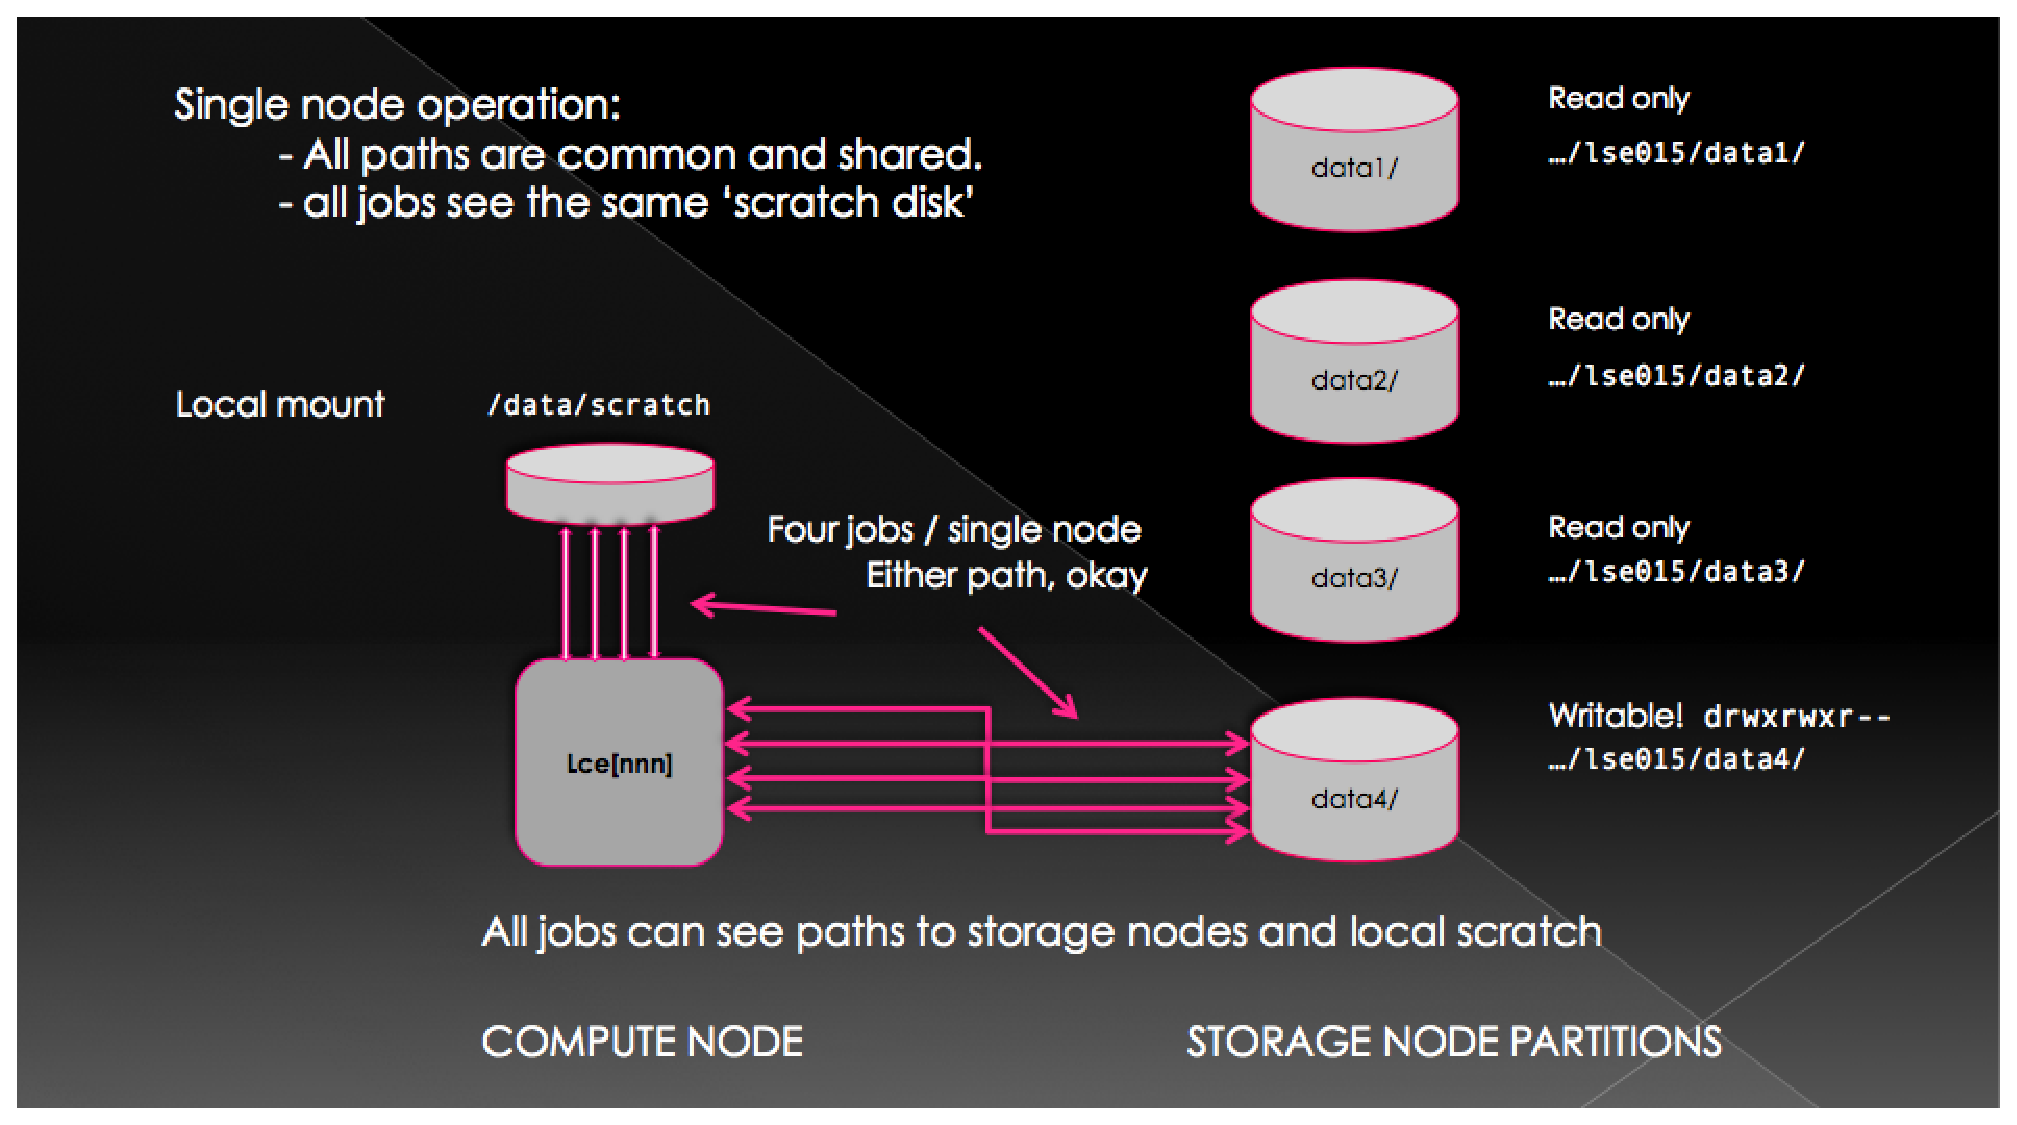
\includegraphics[scale=0.45]{singlenode-0.eps}
  \end{center}
  \caption{Single node operations: all paths are comman and shared}
  \label{fig:singlenode}
\end{figure}

\begin{figure}[htbp] 
  \begin{center}
    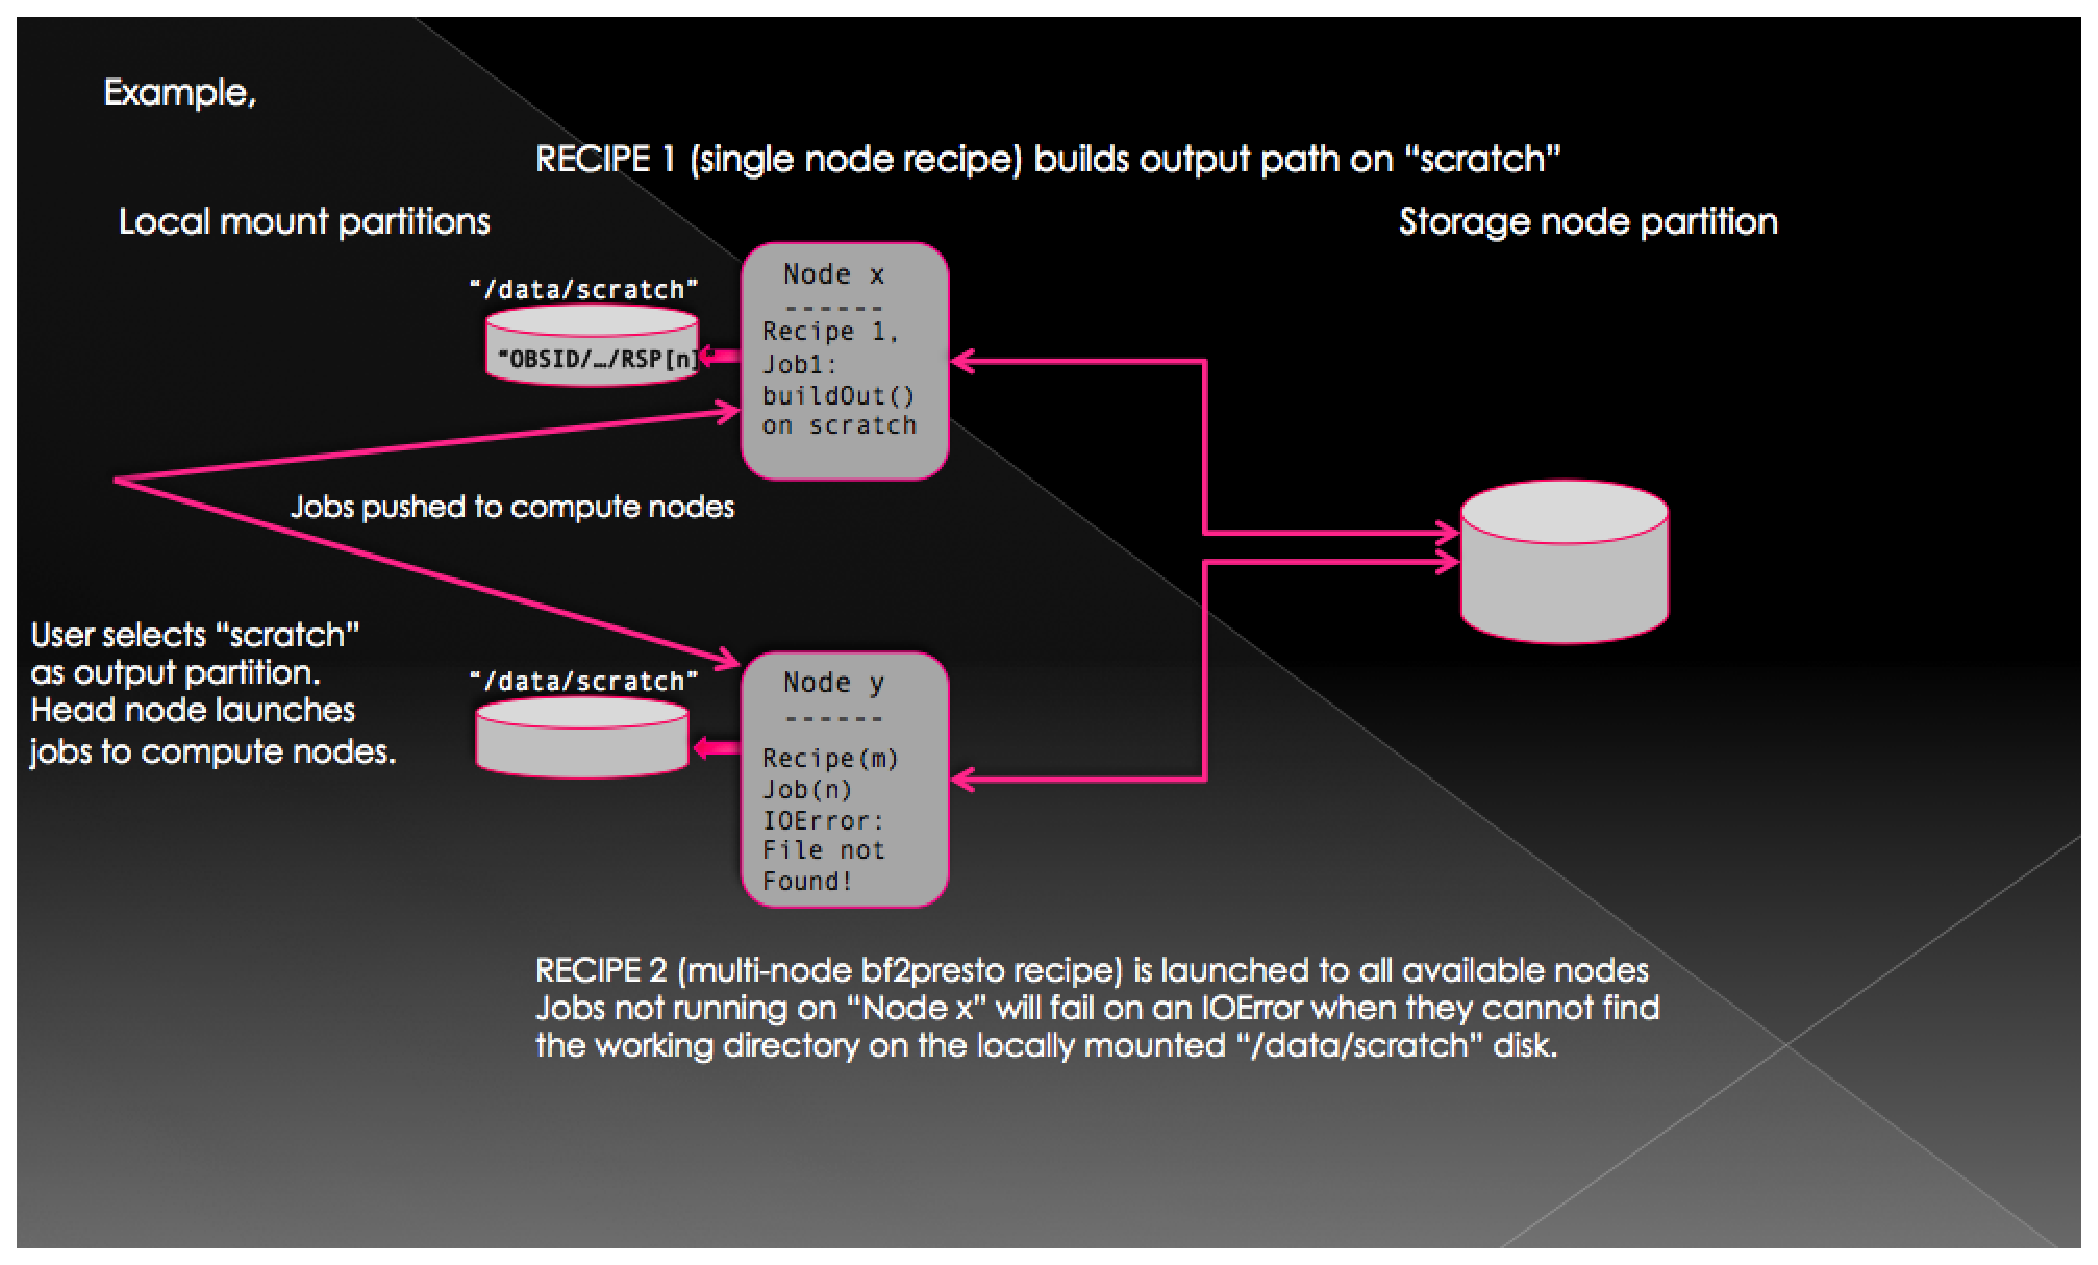
\includegraphics[scale=0.45]{fppPic.eps}
  \end{center}
  \caption{Writing to local disk in a multi-node environment.  Paths
    are common, but not  shared.}
  \label{fig:fpppic}
\end{figure}

The \emph{ad hoc} addition of command line options, and
specifically that of  ``--outputpath'',  was advised against for
the Pulp package.  The driver to have a full and open output path appears
to have been a desire to write to local disk.  User's must understand
that an output path to local disk would \emph{break} the current Pulp
pipeline, unless a user were to restrict pipeline deployment to one
(1) compute node.


Figure \ref{fig:singlenode}  demonstrates that, for a single node --
as the pulsar shell script  would operate on -- all paths to all write
devices are the same for each and every job the pipeline is
running. This is certainly \emph{not} true for framework pipeline
  operations on a multi-node cluster.

The reasons are illustrated in the figure \ref{fig:singlenode}.  What
the figure illustrates can be stated succinctly: when operating in a
multi-node cluster compute environment, locally mounted node disks do
not share comman pathnames.  Writing to local disk would require a
complete redesign and would tend toward the programmatic operatons of
the standard imaging pipeline.

But even if Pulp were refactored to write to local disk.  This still
won't work for the pulsar pipeline as it currently operates.  Speaking
specifically of the ``RSPA'' processing as it is done now, the current
implementation of using symbolic links to ``link in'' all beam formed
data files for ``RSPA'' will not work.  Unless someone knows a way to
create symbolic links across or throughout cluster compute nodes,
``RSPA'' processing cannot be done in a cluster environment.
Restricting the whole pipeline to a single node, which is easily
doable, would allow ``RSPA'' processing to go forward, but then that's
not exactly cluster computing, is it?

\subsection{Future enhancements}
\section{Acknowledgement}
The author wishes to thank John Swinbank for providing vital insight
and levity when the author had none.
\newpage
\section{Appendix A}
\subsection{Pulp Classes: a comprehensive listing of public and private methods}
\label{sec:future-enhancements}
The follow images are a schematic representation of Pulp class
hierarchy.  First, the top level of the package, showing the pipeline
definitions, version and package files. (images: \verb|idle| Path
browser)\footnote{Illustration of an obvious need for a PulpPipeline()
 base class that would supply the python-private ``buildUserEnv()''
 method will follow shortly. However, once the PulpEnv() call is moved to
 the master recipes, this method will be deprecated and expunged.}

\begin{figure}[htbp] 
  \begin{center}
    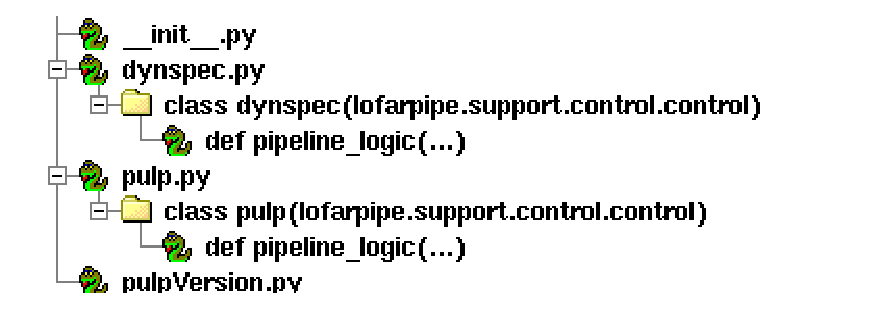
\includegraphics[scale=0.95]{pulpTop.eps} 
  \end{center}
  \caption{Pulp, v1.0, Class Structure and Methods and Functions,
    ``definition'' modules}
\end{figure}

\begin{figure}[htbp] 
  \begin{center}
    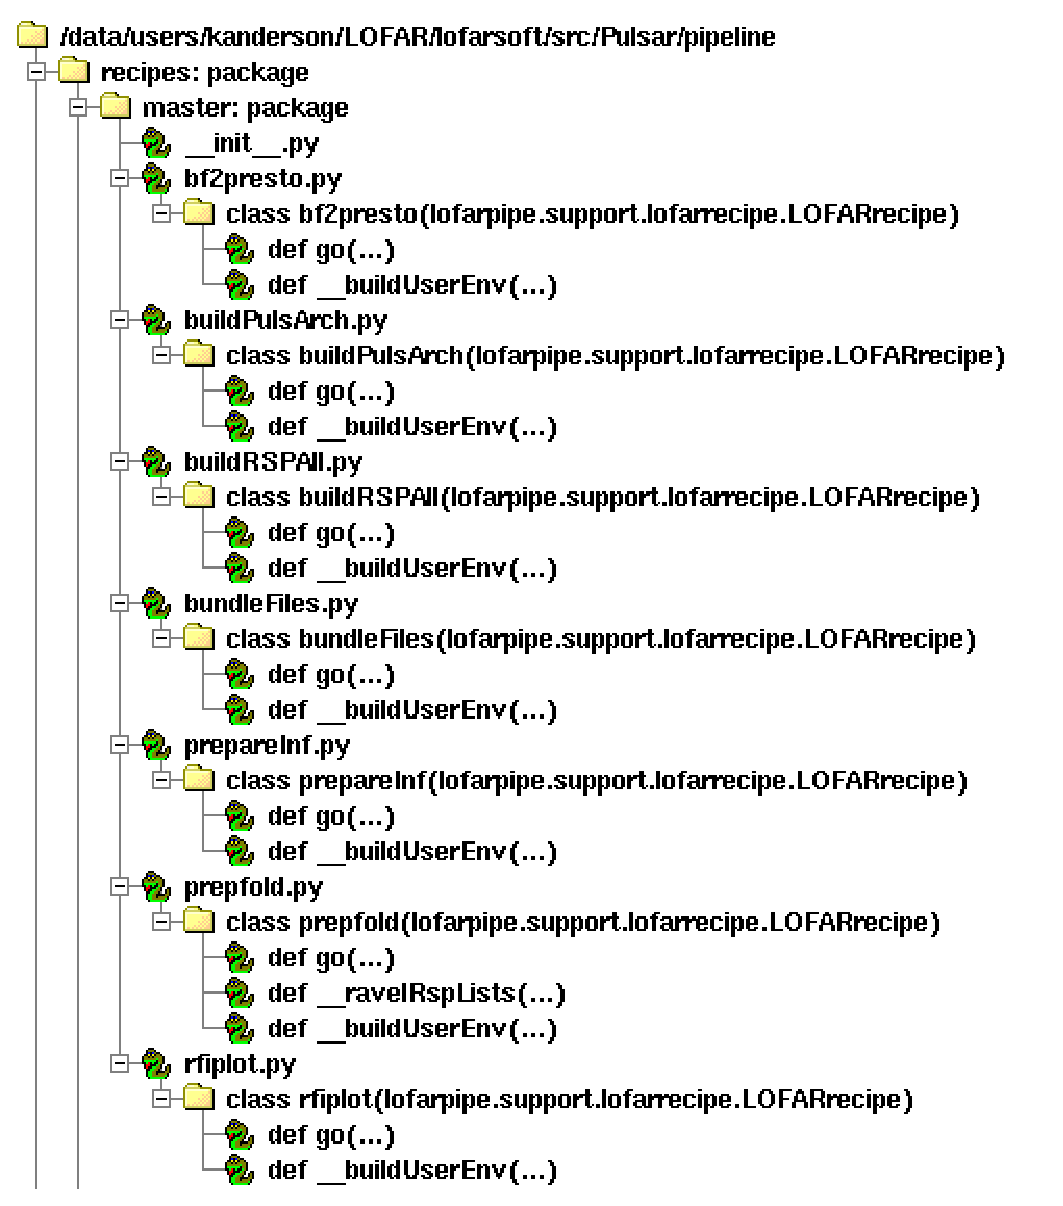
\includegraphics[scale=0.90]{pulpMaster.eps}
  \end{center}
  \caption{Pulp, v1.0, Class Structure, Methods and
    Functions,'``master'' recipe modules}
\end{figure}

\begin{figure}[htbp] 
  \begin{center}
    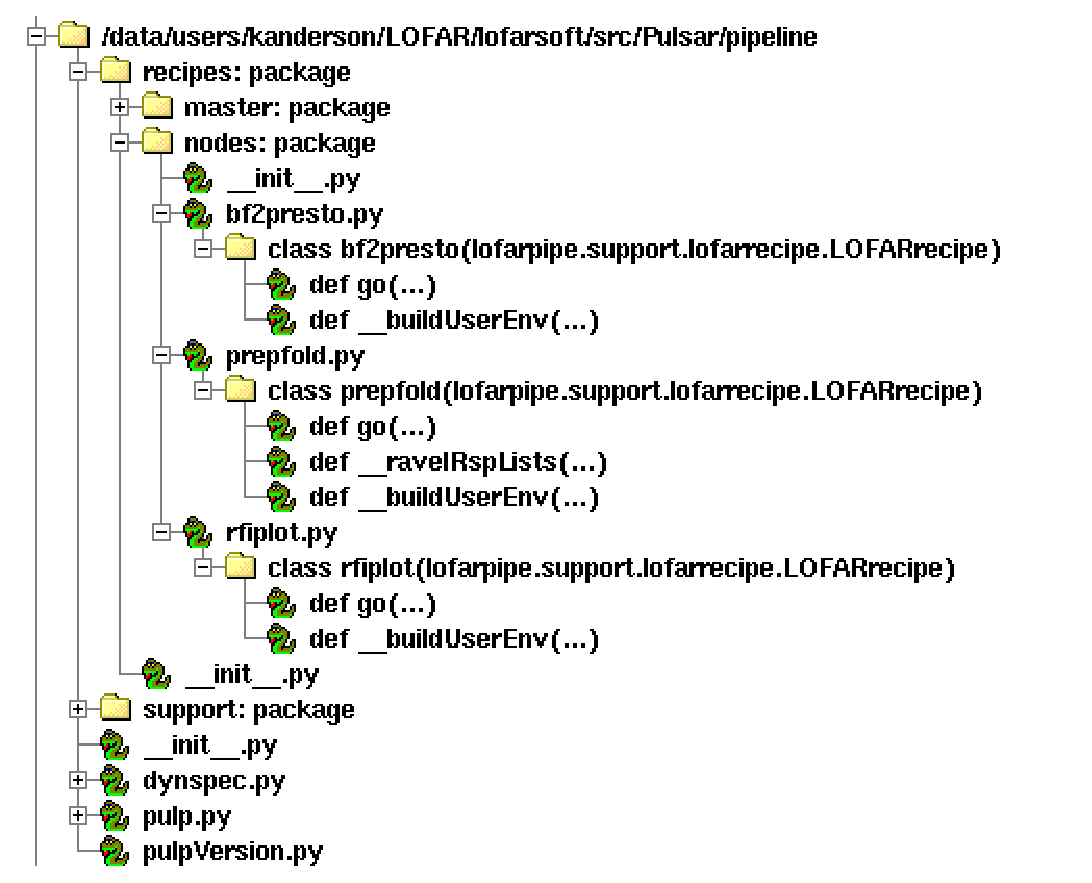
\includegraphics[scale=0.90]{pulpNode.eps}
  \end{center}
  \caption{Pulp, v1.0, Hierarchical Class Structure and Methods,
    ``node'' modules}
  \label{fig:fpppic}
\end{figure}

\begin{figure}[htbp] 
  \begin{center}
    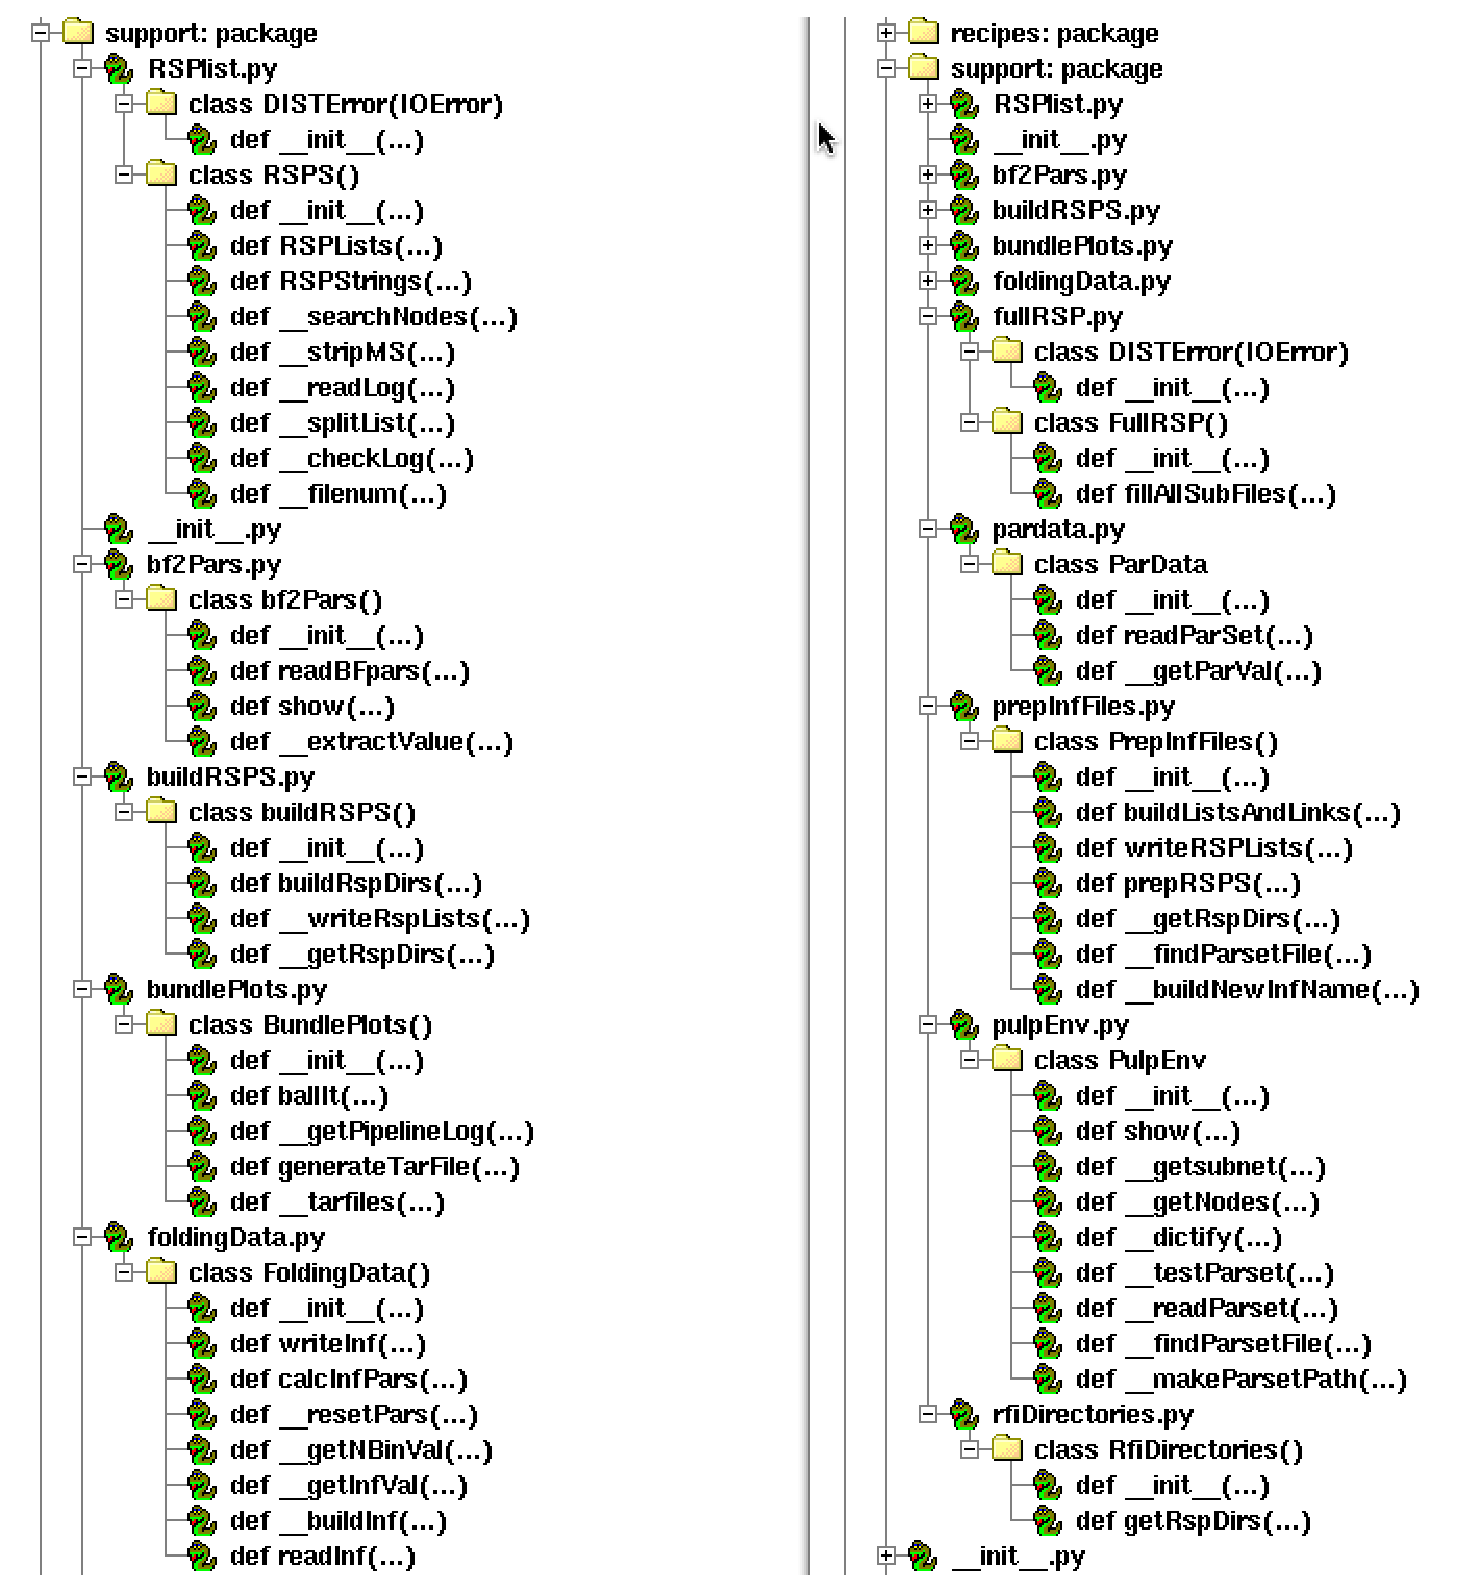
\includegraphics[scale=0.70]{pulpSupport.eps}
  \end{center}
  \caption{Pulp, v1.0, Hierarchical Class Structure and Methods,
    ``support'' modules}
  \label{fig:fpppic}
\end{figure}

\end{document}

